\documentclass{report}
\author{mzx!}
\date{\today}
\newcommand{\ibx}[1]{\framebox[1.1\width]{ #1 }}
\usepackage{amsmath,amssymb}
\usepackage{hyperref}
\usepackage{enumitem} 
\hypersetup{
    colorlinks,
    citecolor=black,
    filecolor=black,
    linkcolor=black,
    urlcolor=black
}

\PassOptionsToPackage{svgnames}{xcolor}
\usepackage{tcolorbox}
\usepackage{lipsum,xcolor,color}
\tcbuselibrary{skins,breakable}
\usetikzlibrary{shadings,shadows}

\definecolor{title_color}{HTML}{ea7dc7}
\definecolor{back_color}{HTML}{f7e8e8}

\newcounter{defboxctr}
\newenvironment{defbox}{%
\refstepcounter{defboxctr}% increment the environment's counter
    \tcolorbox[beamer,%
    noparskip,breakable,
    colback=back_color,colframe=title_color,%
    title={Definition \thedefboxctr}]}%
    {\endtcolorbox}
    \numberwithin{defboxctr}{section}





\title{Econ201 Course Notes}

\begin{document}
\maketitle
\tableofcontents
\chapter{Technology}
\section{Inputs and Outputs}
\begin{defbox}
Inputs to production are called \ibx{Factors of production}\\Physical Capitals

\end{defbox}

\begin{itemize}
\item Land
\item Labor
\item Capital
\begin{itemize}
\item Physical Capital
\begin{itemize}
\item Tractor
\item Buildings
\item Computers
\item Machines of one sort
\end{itemize}
\item Financial Capital
\begin{itemize}
\item Money
\item Stocks
\item Bonds
\end{itemize}
\end{itemize}
\item Raw Materials
\end{itemize}
\section{Technology Constraints (Single Input)}
\begin{defbox}
\paragraph{Production Set}All combinations of inputs and outputs that are technologically feasible
\end{defbox}
\begin{defbox}
\paragraph{Production Function}A function describinig the \textbf{Boundary of Production Set}
$$y=f(x)$$
$x$ = amount of inputs\\$y$ = amount of output
\end{defbox}
Two production functions do not represent the same technology even if one is a \textbf{Monotone Transformation} of the other\\
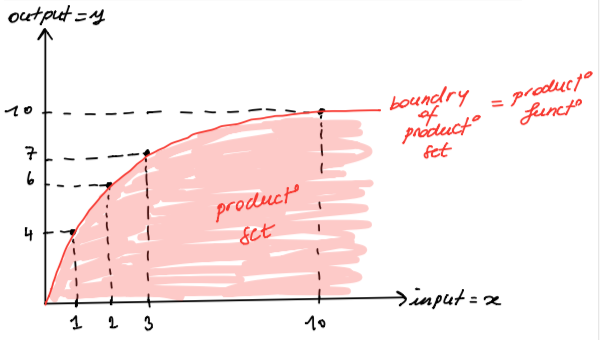
\includegraphics[width = \textwidth]{econ1}
\section{Technology Constraints (Multiple Inputs)}
We consider the case of \textbf{Two Inputs}, the production function $f(x_1,x_2)$ would measure the maximum amount of output $y$ that we could get if we had $x_1$ units of input 1. and $x_2$ units of input 2
\paragraph{Isoquant}
In the two-input case, there is a convenient way to depict production relations known as the isoquant\\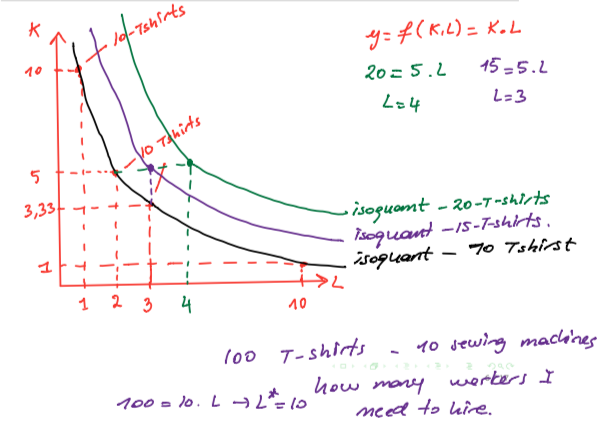
\includegraphics[width = \textwidth]{econ2}

\section{Example of Technology}
\subsection{Fixed Proportion}
$f(x_1,x_2) = min(x_1,x_2)$\\
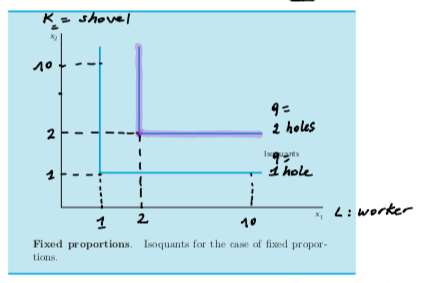
\includegraphics[width = \textwidth]{econ3}
\subsection{Perfect Substitutes}
$f(x_1,x_2) = x_1+x_2$\\
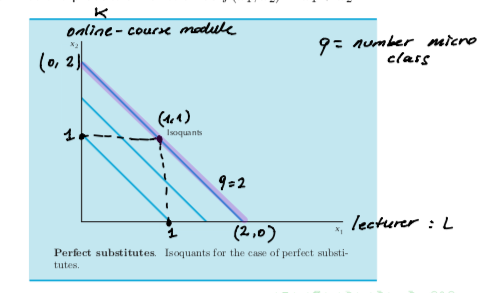
\includegraphics[width = \textwidth]{econ4}
\subsection{Cobb Douglas}
$q=f(x_1,x_2)=Ax_1^ax_2^b$\\A: Scale of Production (how much output we would get if we sued on unit of each input)\\a.b: The amount of output responds to changes in the inputs\\
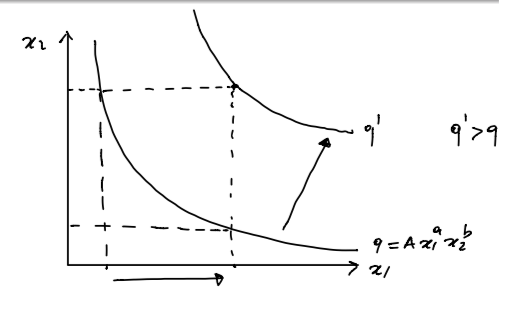
\includegraphics[width = \textwidth]{econ5}
\section{Properties of Technology}
\begin{defbox}
\begin{itemize}
\item Technology is monotonic
\item Technology is convex
\end{itemize}
\end{defbox}
\paragraph{Monotonic}If you increase the amount of at least one of the inputs, it should be possible to produce at least as much output as you were producing originally
\paragraph{Convex}If you have two ways to produce $y$ units of output, $(x_1,x_2)$ and $(z_1,z_2)$, then their weighted average will produce at least $y$ units of output
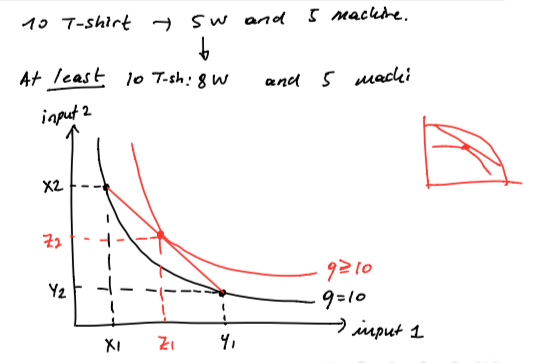
\includegraphics[width = \textwidth]{econ6}
\section{Marginal Product}
\begin{defbox}
Marginal Product of Factor 1
$$MP_1(x_1,x_2)={{\Delta y}\over {\Delta x_1}} = {{f(x_1+\Delta x_1,x_2) - f(x_1,x_2)}\over {\Delta x_1}}$$
or
$$MP_1 = {{\partial y(x_1,x_2)}\over {\partial x_1}}$$
\end{defbox}
$\partial$: Partial Derivative. If $\partial x_1$, then treat $x_2$ as constant value\\$f(x_1,x_2) = 2x_1x_2$,then we have $MP_1 = {{\partial y(x_1,x_2)}\over {\partial x_1}} = 2x_2$
\section{Technical Rate of Substitution}
Suppose that we are operating at $f(x_1,x_2) = y$, at some input level $x_1,x_2$ and output level $y$. We want to adjust $x_1,x_@$ (ie,add $x_1$, less $x_2$), to get the same output level $y$.
\begin{defbox}
$$TRS(x_1,x_2) = {{\Delta x_2}\over {\Delta x_1}} = {{-MP_1(x_1,x_2)}\over {MP_2(x_1,x_2)}}$$
\end{defbox}
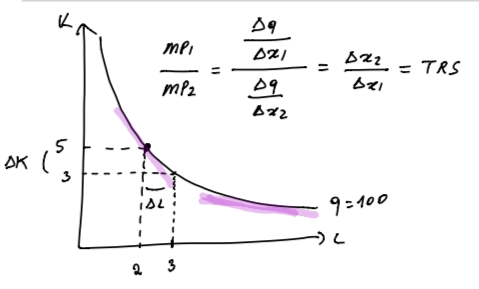
\includegraphics[width = \textwidth]{econ7}
\section{Diminishing Marginal Product}
\paragraph{Law of Diminishing Marginal Product}
As long as we have a monotonic technology, we know that the total output will go up \textbf{As we increase the amount of factor 1}\\But we expect that it will go up at a \textbf{Decreasing Level}
\section{Long Run and Short Run}
\begin{defbox}
\paragraph{Short Run}
\textbf{Some Factors} are fixed
\paragraph{Long Run}
\textbf{All factors} can be varying
\end{defbox}
\section{Returns to scale}
Scale the amount of all inputs up by some constant factor\\This is called the case of \textbf{constant returns to scales}
\begin{defbox}
constant return to scale
$$tf(x_1,x_2) = f(tx_1,tx_2)$$
for some constant $t$
\end{defbox}
\begin{defbox}
Increasing return to scale
$$tf(x_1,x_2) < f(tx_1,tx_2)$$
for some constant $t$
\end{defbox}
\begin{defbox}
Decreasing return to scale
$$tf(x_1,x_2) > f(tx_1,tx_2)$$
for some constant $t$
\end{defbox}
\paragraph{Generalization}
$f(x_1,x_2) = Ax_1^ax_2^b$, then
\begin{itemize}
\item $a + b = 1\to$ constant R.S
\item $a+b>1\to$ Increasing R.S
\item $a+b<1\to$ Decreasing R.S
\end{itemize}
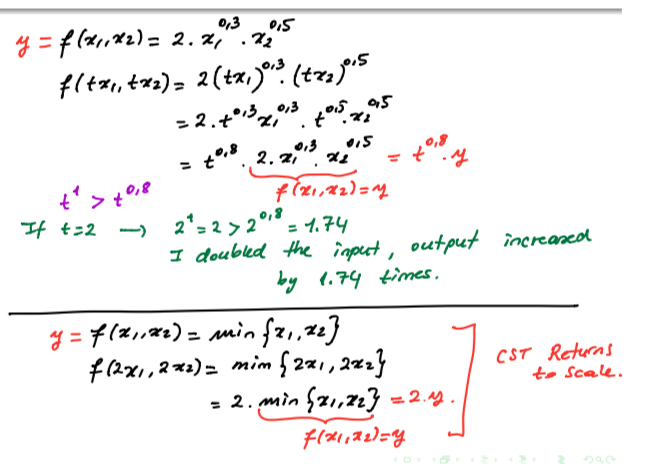
\includegraphics[width = \textwidth]{econ8}
\chapter{Profit Maximization}
\section{Profits}
\begin{defbox}
\paragraph{Profits}
are defined as \textbf{Revenues} minus \textbf{Cost}
$$\pi = p\times q-w_1x_1-w_2x_2$$
\begin{itemize}
\item $p$ = price of output
\item $q$ = output
\item $w_1$ = price of input 1
\item $w_2$ = price of input 2
\end{itemize}
\end{defbox}
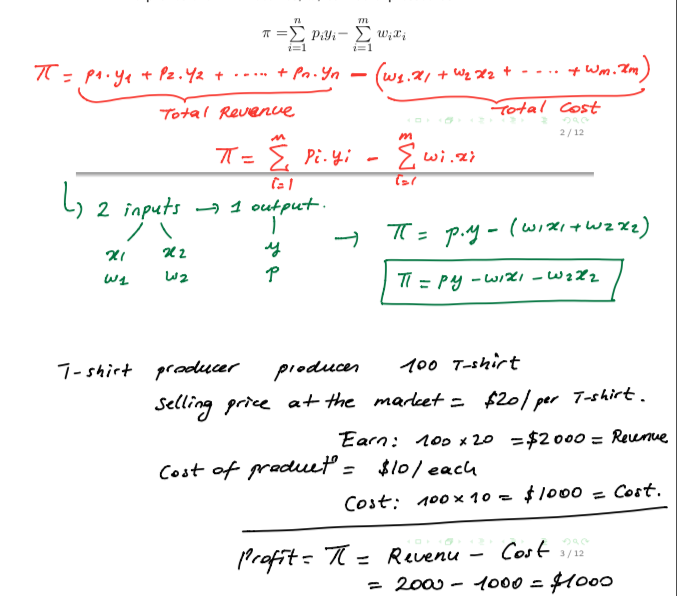
\includegraphics[width = 0.7\textwidth]{econ9}
\section{Short-Run Profit Maximization}
\begin{defbox}
$$pMP_1(x_1^*,x_2)=w_1$$

\begin{itemize}
\item $p$ = Output Price
\item $MP_1$ = Marginal Product of factor 1
\item $x_1^*$ = the profit\_maximizing choice for factor 1
\item $w_1$ = the price of factor 1
\end{itemize}

\end{defbox}
\paragraph{Recall}

\paragraph{Generalized}
\begin{itemize}
\item $pMP_1>w_1\to$ Should Increase $x_1$
\item $pMP_1=w_1\to$ Keep $x_1$
\item $pMP_1<w_1\to$ Should Decrease $x_1$
\end{itemize}
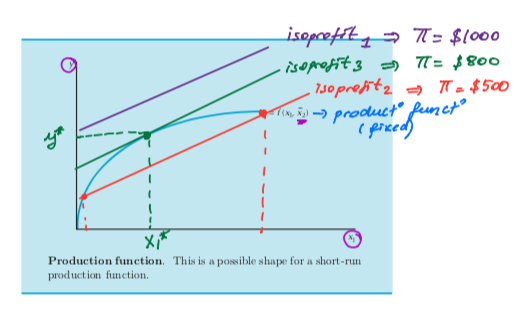
\includegraphics[width = \textwidth]{econ10}
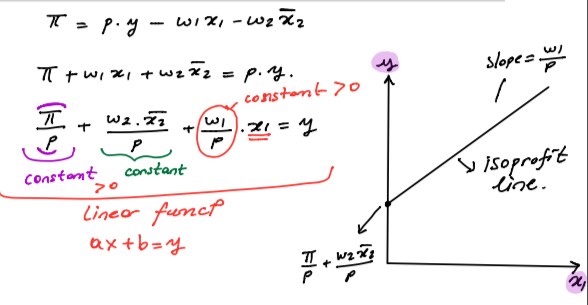
\includegraphics[width = \textwidth]{econ11}
\subsection{Tangency Condition}
The slope of the production function should equal the slope the isoprofit line
$$MP_1 = {w_1\over p}$$
or
$$pMP_1=w_1$$
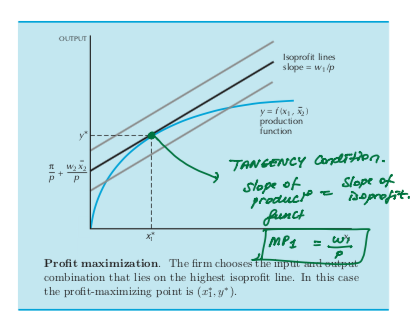
\includegraphics[width = \textwidth]{econ12}
\section{Long-Run Profit Maximization}
In the Long-Run, we are free to choose \ibx{Level of All Inputs}
\begin{defbox}
Long-Run Profit-Maximization
$$\max_{x_1,x_2} pf(x_1,x_2)-w_1x_1-w_2x_2$$
\end{defbox}
\paragraph{Generalize}
\begin{itemize}
\item $pMP_1(x_1^*,x_2^*)=w_1$
\item $pMP_2(x_1^*,x_2^*)=w_2$
\end{itemize}
\paragraph{In Long Run}
Additional Revenue from $x_i$ = Additional Cost of $x_i$
\section{Inverse Factor Demand Curves}
\paragraph{Factor Demand Curves}
measures the relationship between the \ibx{price of a factor} and the \ibx{profit-maximizing choice} of that factor
\end{document}
\paragraph{Inverse Factor Demand Curve}
measures what the factor prices must be for some given quantity  of inputs to be demanded
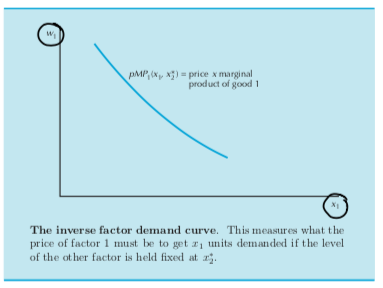
\includegraphics[width = \textwidth]{econ13}